%作者:汪斐然
%模板用途:模式识别报告
%时间:2021年3月


%这是一份基于《2020-2021模式识别期末提交模板》Word版制作的Latex模板。用于方昱春老师的模式识别课程报告。
%文档中对Latex的各种使用方式都准备了样例并进行备注,包括标题设置、图表添加、文献引用以及字体设置等。
%参考文献格式和Word版存在一定的区别,使用的是IEEETR格式。是IEEE期刊使用的参考文献引用标准。
%参考文献选择使用IEEETR格式的原因在于,可以在文章中对参考文献进行超链接索引。
%希望这份模板可以帮助同学们快速上手Latex,制作漂亮的课程报告;可以在同学们之后的研究学习过程中成为学术论文的参考模板。

%Latex工具:本地编辑平台:TexWorks;在线编辑平台:Overleaf(推荐)

%Latex快速入门教程:
%1、https://muyuuuu.github.io/2018/11/07/Brief-introduction-to-LaTex/
%2、https://liam.page/2014/09/08/latex-introduction/

%Latex快速辅助工具使用说明:
%快速绘制表格工具:https://www.tablesgenerator.com/
%快速生成公式工具:https://mathpix.com/

%%%%%%%%%%%%%%%%%%%%%%%%%%%%%环境配置%%%%%%%%%%%%%%%%%%%%%%%%%%%%%%%%%%

\documentclass{article}
\usepackage[UTF8]{ctex}
\usepackage[left=3.18cm,right=3.18cm,top=2.54cm,bottom=2.54cm]{geometry}
\geometry{a4paper}

%附录包
\usepackage{appendix} 
\usepackage{listings}
\usepackage{cite}
%代码格式
\usepackage{xcolor}
\lstset{
    numbers=left, 
    numberstyle= \tiny, 
    keywordstyle= \color{ blue!70},
    commentstyle= \color{red!50!green!50!blue!50}, 
    frame=shadowbox, % 阴影效果
    rulesepcolor= \color{ red!20!green!20!blue!20} ,
    escapeinside=``, % 英文分号中可写入中文
    xleftmargin=2em,xrightmargin=2em, aboveskip=1em,
    framexleftmargin=2em
} 
\usepackage{algorithm}
\usepackage{algpseudocode}
\renewcommand{\algorithmicrequire}{\textbf{Input:}}  % Use Input in the 
\renewcommand{\algorithmicensure}{\textbf{Output:}} % Use Output in the 

%数学
\usepackage{amsmath}
\usepackage{amsthm}

%图片
\usepackage{graphicx} %添加图片

%字体、格式设置
\usepackage{subfigure}
\usepackage{float}
\renewcommand{\vec}[1]{\boldsymbol{#1}} % 生产粗体向量,而不是带箭头的向量
\usepackage{amssymb}
\usepackage{booktabs} % excel导出的大表格
\usepackage{hyperref}
\usepackage{titlesec}%设置字体的包
%可选字体:
% \noindent 中文字体(默认宋体)\\
% \fangsong 中文字体(仿宋) \songti 中文字体(宋体) \lishu 中文字体(隶书) \heiti 中文字体(黑体)\\
% \CJKfamily{zhkai} 中文字体(楷书) \CJKfamily{zhyou} 中文字体(幼圆) \CJKfamily{zhyahei} 中文字体(微软雅黑)\\

%调整图表标题的字体样式
\usepackage{caption}
\captionsetup{font={small,bf}} 

%新定义
\newtheorem{definition}{定义} %中文
\newtheorem{lemma}{引理}
\newtheorem{theorem}{定理}
\DeclareMathOperator{\Ima}{Im}%定义新符号
\DeclareMathOperator{\Rank}{rank}%定义求秩算子

\usepackage{pdfpages}


%设置标题,作者
\title{\textbf{基于XGBoost与SVM的网络入侵检测系统:以UNSW-NB15数据集为例}}
\author{
王宇飞(22122850)
}

%%%%%%%%%%%%%%%%%%%%%%%%%%%%%%%正文%%%%%%%%%%%%%%%%%%%%%%%%%%%%%%%%%%
%\songti(宋体)设置全文字体,可改为\heiti(黑体),\fangsong(仿宋)
\begin{document} \songti

% \centerline{\heiti\zihao{2}{上海大学2024 $ \sim $ 2025学年}}
\vspace{10bp}
\centerline{\heiti\zihao{2}{课程报告成绩评价表}}

\vskip 2cm

\begin{flushleft}
	\zihao{3}
	{\heiti{课程名称:}}      
	{\heiti\underline{\quad\textbf{《模式识别》}\quad}}
        {\heiti{课程编号:}}      
	{\heiti\underline{\quad\textbf{08306089}\hspace{1cm}}}   
                \\
	\vspace{20bp}
	{\heiti{ {报告名称:}}}      
	{\heiti\underline{\hspace{2.8cm}\textbf{}\hspace{8.8cm}}}              
                \\
	\vspace{20bp}
	{\heiti{{姓}\quad\quad{名:}}}      
	{\heiti\underline{\quad\quad\quad\quad\textbf{哇}\quad\quad\quad\quad}}
        {\heiti{{学}\quad\quad{号:}}}      
	{\heiti\underline{\quad\quad\quad\textbf{}\quad\quad\quad\quad}} 
                \\
        \vspace{20bp}
	{\heiti{ {报告评语:}}} 
                \\
        \vspace{15bp}
        \fbox{%
            \parbox{1.04\textwidth}{%
                \begin{center}
                    \\\quad 
                    \\\quad 
                \end{center}
                }%
            }
        
        \vspace{20bp}
	{\heiti{{报告成绩:}}} 
\\
\vspace{5bp}
\begin{table}[htbp]
\setlength{\tabcolsep}{0.37cm}
\begin{tabular}{|cl|cl|cll|c|}
\hline
\multicolumn{2}{|c|}{方案设计(20分)}                                                                                                                      & \multicolumn{2}{c|}{验收(20分)}                                                                                                                         & \multicolumn{3}{c|}{书面报告(60分)}                                                                                                                      & \multirow{2}{*}{总分}   \\ \cline{1-7}
\multicolumn{1}{|c|}{\begin{tabular}[c]{@{}c@{}}可行性\\ (10分)\end{tabular}} & \multicolumn{1}{c|}{\begin{tabular}[c]{@{}c@{}}创新性\\ (10分)\end{tabular}} & \multicolumn{1}{c|}{\begin{tabular}[c]{@{}c@{}}规范性\\ (10分)\end{tabular}} & \multicolumn{1}{c|}{\begin{tabular}[c]{@{}c@{}}演示效果\\ (10分)\end{tabular}} & \multicolumn{1}{c|}{\begin{tabular}[c]{@{}c@{}}规范性\\ (20分)\end{tabular}} & \multicolumn{1}{c|}{\begin{tabular}[c]{@{}c@{}}完整性\\ (20分)\end{tabular}} & \multicolumn{1}{c|}{\begin{tabular}[c]{@{}c@{}}科学性\\ (20分)\end{tabular}} &                       \\ \hline
\multicolumn{1}{|l|}{}                                                    &                                                                          & \multicolumn{1}{l|}{}                                                    &                                                                           & \multicolumn{1}{l|}{}                                                    & \multicolumn{1}{l|}{}                                                    &           \rule{0pt}{3\normalbaselineskip}                                                               & \multicolumn{1}{l|}{} \\ \hline

\end{tabular}
\end{table}

\end{flushleft}

\vspace{20bp}
\leftline{\heiti\zihao{3}{任课教师:}}
\vspace{20bp}
\leftline{\heiti\zihao{3} {评阅日期:     \quad\quad\quad     年  \quad\quad  月  \quad\quad  日         }} %调用封面文件
% 插入封面

\date{}
\maketitle


%%%%%%%%%%%%%%%%%%%%%%摘要%%%%%%%%%%%%%%%%%%%%%%%%%%%%%
%由摘要和关键词两部分组成
\begin{center}
\setlength{\textwidth}{15cm}
\parbox{\textwidth}{
\textbf{摘要:}200字左右,应包括目的、方法、结果和结论等要素。目的目的目的目的目的目的目的目的目的目的目的目的目的目的目的目的目的目的。方法方法方法方法方法方法方法方法方法方法方法方法方法方法方法方法。结果结果结果结果结果结果结果结果结果结果结果结果结果结果结果结果结果结果结果结果结果结果。结论结论结论结论结论结论结论结论结论结论结论结论结论结论结论结论结论。
% \newline
%   \textbf{关键词:}图像分类, K近邻, 支持向量机, 数据增强
  }
\end{center}

%%%%%%%%%%%%%%%%%%%%%%目录%%%%%%%%%%%%%%%%%%%%%%%%%%%%%
% \newpage
% \tableofcontents
% \newpage
%%%%%%%%%%%%%%%%%%%%%%%%%%%%%%%%%%%%%%%%%%%%%%%%%%%%%%%%
%一级标题
\section{引言}
%%%%%%%%%%%%%%%%%%%%%%%%%%%
%二级标题
\subsection{提出问题(300-500字)}
%三级标题
\subsubsection{三级标题}
正文正文正文正文正文正文正文正文正文正文,正文正文正文正文正文正文正文正文正文正文。正文正文正文正文正文正文正文正文正文正文正文,正文正文正文正文正文正文正文正文正文正文。正文正文正文正文正文正文正文正文正文正文正文,正文正文正文正文正文正文正文正文正文正文。\cite{ref1}

\subsubsection{三级标题}
正文正文正文正文正文正文正文正文正文正文,正文正文正文正文正文正文正文正文正文正文。正文正文正文正文正文正文正文正文正文正文正文,正文正文正文正文正文正文正文正文正文正文。正文正文正文正文正文正文正文正文正文正文正文,正文正文正文正文正文正文正文正文正文正文。

%%%%%%%%%%%%%%%%%%%%%%%%%%%
\subsection{求解方案分析(300-500字)}
正文正文正文正文正文正文正文正文正文正文,正文正文正文正文正文正文正文正文正文正文。正文正文正文正文正文正文正文正文正文正文正文,正文正文正文正文正文正文正文正文正文正文。正文正文正文正文正文正文正文正文正文正文正文,正文正文正文正文正文正文正文正文正文正文。

%%%%%%%%%%%%%%%%%%%%%%%%%%%
\subsection{论文概述(200字)}
正文正文正文正文正文正文正文正文正文正文,正文正文正文正文正文正文正文正文正文正文。正文正文正文正文正文正文正文正文正文正文正文,正文正文正文正文正文正文正文正文正文正文。正文正文正文正文正文正文正文正文正文正文正文,正文正文正文正文正文正文正文正文正文正文。

%%%%%%%%%%%%%%%%%%%%%%%%%%%%%%%%%%%%%%%%%%%%%%%%%%%%%%%%


\section{数据处理与模型构建}
%%%%%%%%%%%%%%%%%%%%%%%%%%%
\subsection{UNSW-NB15数据集}
UNSW-NB15数据集是由澳大利亚新南威尔士大学堪培拉分校(UNSW Canberra)的网络靶场实验室
(Cyber Range Lab)使用IXIA PerfectStorm工具生成的。该数据集旨在模拟现代网络环境中的正常活
动和合成攻击行为,从而为网络入侵检测研究提供高质量的实验数据。通过Tcpdump工具捕获了100 GB的原始
网络流量数据(如Pcap文件),并进一步处理生成了包含多种攻击类型和正常流量的结构化数据集。在这项工作中,UNSW-NB15 
数据集中共有 257,673 个
数据实例,其中包括 175,341 个训练数据实例和 82,332 个测
试数据实例。
\subsubsection{数据集分类情况}
UNSW-NB15数据集涵盖了一种正常流量类型和九种主要的攻击类型,包括Fuzzers、Analysis、Backdoors、DoS(拒绝服务攻击)
、Exploits、Generic、Reconnaissance(侦察攻击)、Shellcode和Worms。这些攻击类型覆盖了广泛的网络威
胁,能够有效支持入侵检测系统的训练与评估。
\begin{table}[H]
  \caption{UNSW-NB15数据集中的标签及其含义}
  \label{table:sample} % 将label放在caption之后
  \begin{center}
    \resizebox{\textwidth}{!}{  % 按页面宽度缩放表格
  \begin{tabular}{|l|l|l|} % 使用 r 表示右对齐
\hline
ID & Type           & Description                                                                                                            \\ \hline
1  & Normal         & Natural transaction data.                                                                                              \\ \hline
2  & Analysis       & An attack to invade web applications through emails ports or web scripts.                                              \\ \hline
3  & Backdoor       & A covert attempt to circumvent normal authentication measures or other processes by allowing for secure remote access. \\ \hline
4  & DoS            & A malicious attempt to disrupt the computer resources by attacking memory.                                             \\ \hline
5  & Exploits       & An instruction to take advantage of bugs or errors caused by unintentional behavior on the network.                    \\ \hline
6  & Fuzzers        & An attack to crash the system by inputting a lot of random data.                                                       \\ \hline
7  & Generic        & A technique to clash the block-cipher configuration by using hash functions.                                           \\ \hline
8  & Reconnaissance & A probe to evade network security controls by collecting relevant information.                                         \\ \hline
9  & Shellcode      & A piece of code that is executed to exploit software vulnerabilities.                                                  \\ \hline
10 & Worms          & A set of virus code which can add itself to computer system or other programs.                                         \\ \hline
\end{tabular}
    }
\end{center}
\end{table}
\subsubsection{数据集特征情况}
本数据集的257,673项数据中,共含有49个特征(包含类别标签),其中所有特征被分为 6 组,
包括流量、基础、内容、时间、附加生成和标记特征。特
别地,特征 1 至 35 代表从数据包中集成收集的信息。附
加生成的特征进一步分为通用特征和连接特征两部分。特
征 36 至 39 被视为连接特征,而特征 40 至 47 被视为
通用特征。特征 48 至 49 为标记特征。
\begin{table}[H]
  \caption{UNSW-NB15数据集中的特征}
  \label{table:feature} % 将label放在caption之后
  \begin{center}
    \resizebox{\textwidth}{!}{  % 按页面宽度缩放表格
    \begin{tabular}{|l|l|l|l|l|l|l|l|}
      \hline
      No. & Name   & No. & Name          & No. & Name                & No. & Name                \\ \hline
      1   & srcip  & 14  & service       & 27  & Sjit                & 40  & ct\_ftp\_cmd        \\ \hline
      2   & sport  & 15  & Sload         & 28  & Djit                & 41  & ct\_srv\_src        \\ \hline
      3   & dstip  & 16  & Dload         & 29  & Stime               & 42  & ct\_srv\_dst        \\ \hline
      4   & dsport & 17  & Spkts         & 30  & Ltime               & 43  & ct\_dst\_ltm        \\ \hline
      5   & proto  & 18  & Dpkts         & 31  & Sintpkt             & 44  & ct\_src\_ ltm       \\ \hline
      6   & state  & 19  & swin          & 32  & Dintpkt             & 45  & ct\_src\_dport\_ltm \\ \hline
      7   & dur    & 20  & dwin          & 33  & tcprtt              & 46  & ct\_dst\_sport\_ltm \\ \hline
      8   & sbytes & 21  & stcpb         & 34  & synack              & 47  & ct\_dst\_src\_ltm   \\ \hline
      9   & dbytes & 22  & dtcpb         & 35  & ackdat              & 48  & attack\_cat         \\ \hline
      10  & sttl   & 23  & smeansz       & 36  & is\_sm\_ips\_ports  & 49  & Label               \\ \hline
      11  & dttl   & 24  & dmeansz       & 37  & ct\_state\_ttl      &     &                     \\ \hline
      12  & sloss  & 25  & trans\_depth  & 38  & ct\_flw\_http\_mthd &     &                     \\ \hline
      13  & dloss  & 26  & res\_bdy\_len & 39  & is\_ftp\_login      &     &                     \\ \hline
  \end{tabular}
    }
  \end{center}
\end{table}

\subsubsection{数据分布情况}
由图\ref{fig:combined}可以发现,数据集中各类别的条目数量分布并不均衡,这有可能导致模型在训练和测试过程中对于少数类别的识别效果不佳。
因此,在训练与评估模型时,需要采取一些策略来处理数据集中的类别不平衡问题。
\begin{figure}[H]
  \centering
  \begin{minipage}[b]{0.45\textwidth}
      \centering
      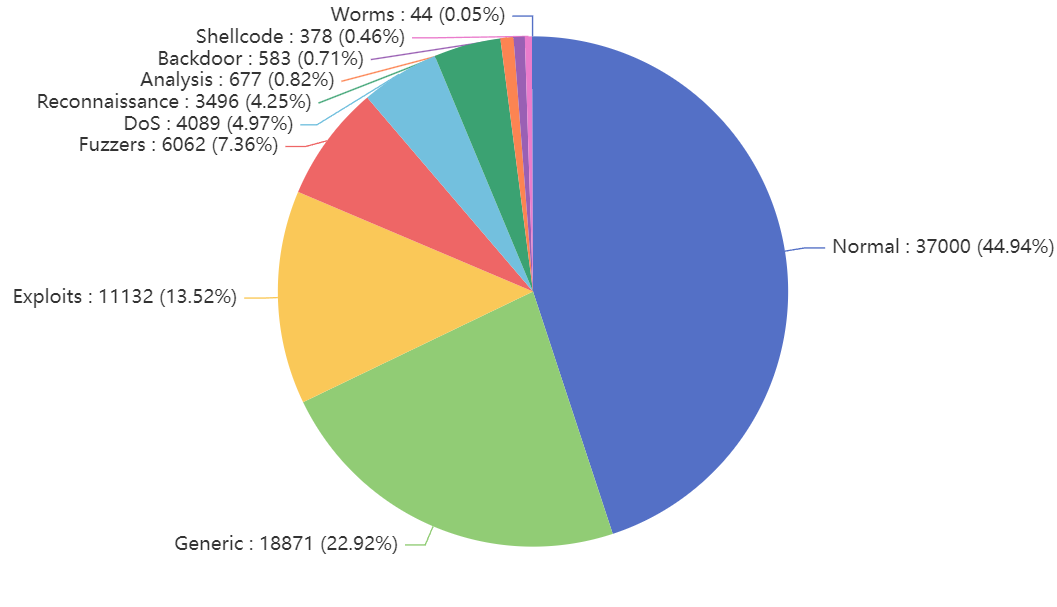
\includegraphics[width=\textwidth]{./png/acc2.png}
      % \caption{测试集攻击分类占比情况}
      \label{fig:test_set}
  \end{minipage}
  \hspace{0.05\textwidth}  % 图像之间的水平间距
  \begin{minipage}[b]{0.45\textwidth}
      \centering
      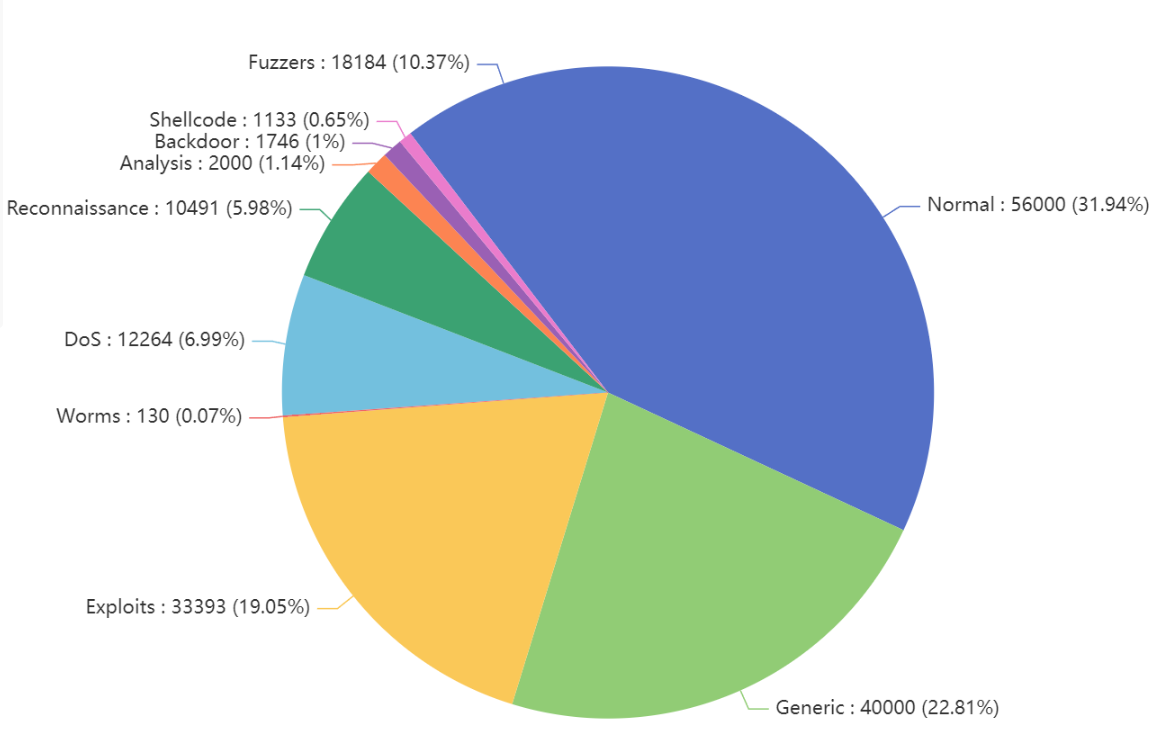
\includegraphics[width=\textwidth]{./png/acc1.png}
      % \caption{训练集攻击分类占比情况}
      \label{fig:train_set}
  \end{minipage}
  \caption{训练集与测试集攻击分类占比情况}
  \label{fig:combined}
\end{figure}

\subsection{数据预处理}

\subsubsection{数据完整度检验}
由于数据量过大,为了提高数据处理效率,我们首先对数据集进行了数据完整性检验。如图\ref{fig:full}所示,
service列出现超过半数的数据缺失,因此我们选择从数据集中移除该列数据,防止对后续的模型训练造成影响。
\begin{figure}[htpb]
  \centering
  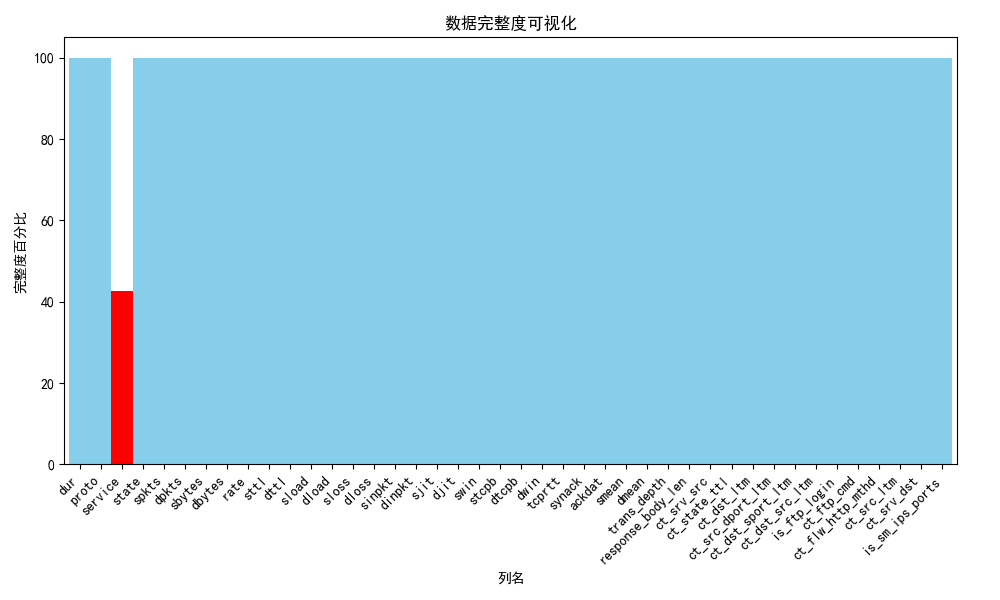
\includegraphics[width=0.9\textwidth]{./png/full.png}
  \caption{数据完整性}
  \label{fig:full}
\end{figure}
\subsubsection{字符串标签列处理}
在数据集中,有一些列的数据类型为字符串,例如proto、state等。
为了方便后续的模型训练,我们选择独热编码将这些字符串标签列进行了数值化处理。
\subsubsection{数据标准化}

首先,我们计算了原始数据的偏度值。偏度是衡量数据分布对称性的一种统计量。
若偏度值接近0,则表示数据分布接近正态分布;若偏度值显著大于0或小于0,则说明数据分布偏向右侧或左侧。
由图\ref{fig:skew}可知,原始数据的偏度值存在显著的偏斜,显示出非常强烈的右偏分布,
这些强烈的偏斜可能会对基于正态分布假设的模型(如线性回归)产生负面影响,因此需要进行标准化处理。

为了解决数据的偏斜问题,我们对数据进行了对数转换。对数转换是一种常用的标准化方法,它可以有效地减少正偏分布的影响,并使数据趋向正态分布。
通过对原始数据进行对数转换后,数据偏度值明显降低,大多数特征的偏度接近零,表示数据分布趋向正态,显著改善了该特征的分布。
\begin{figure}[H]
  \centering
  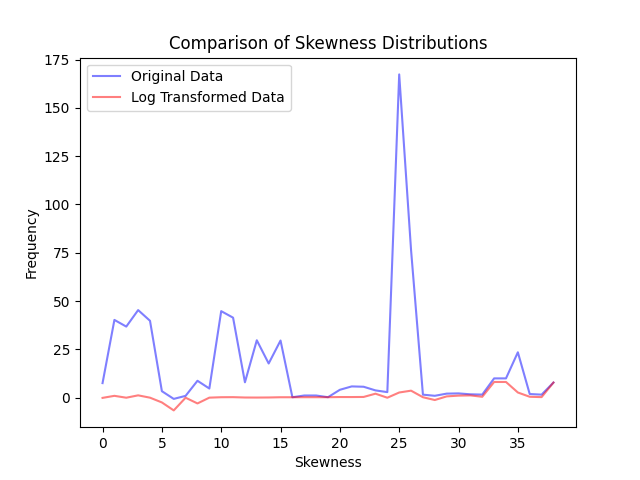
\includegraphics[width=0.7\textwidth]{./png/skewness.png}
  \caption{数据偏度量}
  \label{fig:skew}
\end{figure}

%%%%%%%%%%%%%%%%%%%%%%%%%%%%%%%%%%%%%%%%%%%%%%%%%%%%%%%%


\section{算法实现描述}
正文正文正文正文正文正文正文正文正文正文,正文正文正文正文正文正文正文正文正文正文。正文正文正文正文正文正文正文正文正文正文正文,正文正文正文正文正文正文正文正文正文正文。正文正文正文正文正文正文正文正文正文正文正文,正文正文正文正文正文正文正文正文正文正文。

\subsection{算法总体框架(>500字)}
正文正文正文正文正文正文正文正文正文正文,正文正文正文正文正文正文正文正文正文正文。正文正文正文正文正文正文正文正文正文正文正文,正文正文正文正文正文正文正文正文正文正文。正文正文正文正文正文正文正文正文正文正文正文,正文正文正文正文正文正文正文正文正文正文


\subsection{改进一及分析(>500字)}
正文正文正文正文正文正文正文正文正文正文,正文正文正文正文正文正文正文正文正文正文。正文正文正文正文正文正文正文正文正文正文正文,正文正文正文正文正文正文正文正文正文正文。正文正文正文正文正文正文正文正文正文正文正文,正文正文正文正文正文正文正文正文正文正文。

\subsection{改进二及分析(>500字)}
正文正文正文正文正文正文正文正文正文正文,正文正文正文正文正文正文正文正文正文正文。正文正文正文正文正文正文正文正文正文正文正文,正文正文正文正文正文正文正文正文正文正文。正文正文正文正文正文正文正文正文正文正文正文,正文正文正文正文正文正文正文正文正文正文。


%%%%%%%%%%%%%%%%%%%%%%%%%%%%%%%%%%%%%%%%%%%%%%%%%%%%%%%%

\begin{equation}\label{eq:sample}
  P(f)=\frac{1}{T} \mid 2 \pi f A \exp \left[-\frac{(2 \pi f \sigma)^{2}}{2}\right]^{2}
  \end{equation}
\section{实验描述}
\subsection{实验数据和实验方案 (>500字)}
正文正文正文正文正文正文正文正文正文正文,正文正文正文正文正文正文正文正文正文正文。正文正文正文正文正文正文正文正文正文正文正文,正文正文正文正文正文正文正文正文正文正文。正文正文正文正文正文正文正文正文正文正文正文,正文正文正文正文正文正文正文正文正文正文。

\subsection{实验一及结果分析 (>500字)}
正文正文正文正文正文正文正文正文正文正文,正文正文正文正文正文正文正文正文正文正文。正文正文正文正文正文正文正文正文正文正文正文,正文正文正文正文正文正文正文正文正文正文。正文正文正文正文正文正文正文正文正文正文正文,正文正文正文正文正文正文正文正文正文正文。

\subsection{实验二及结果分析 (>500字)}
正文正文正文正文正文正文正文正文正文正文,正文正文正文正文正文正文正文正文正文正文。正文正文正文正文正文正文正文正文正文正文正文,正文正文正文正文正文正文正文正文正文正文。正文正文正文正文正文正文正文正文正文正文正文,正文正文正文正文正文正文正文正文正文正文。

%%%%%%%%%%%%%%%%%%%%%%%%%%%%%%%%%%%%%%%%%%%%%%%%%%%%%%%%

% \begin{table}[H]
% \caption{表题标题}
% \begin{center}\label{table:sanple}

% \begin{tabular}{|c|r|r|r|}
% \hline
%     & \multicolumn{1}{c|}{速度/(m.s-1)} & \multicolumn{1}{c|}{时间/s} & \multicolumn{1}{c|}{频率/kHz} \\ \hline
% 第一次 &                                 &                           &                             \\ \hline
% 第二次 &                                 &                           &                             \\ \hline
% 第三次 &                                 &                           &                             \\ \hline
% \end{tabular}
  
% \end{center}
% \end{table}
\section{结论(500字)}
正文正文正文正文正文正文正文正文正文正文,正文正文正文正文正文正文正文正文正文正文。正文正文正文正文正文正文正文正文正文正文正文,正文正文正文正文正文正文正文正文正文正文。正文正文正文正文正文正文正文正文正文正文正文,正文正文正文正文正文正文正文正文正文正文。

%%%%%%%%%%%%%%%%%%%%%%%%%%%%%%%%%%%%%%%%%%%%%%%%%%%%%%%%
\section{学习体会和建议(300字)}
正文正文正文正文正文正文正文正文正文正文,正文正文正文正文正文正文正文正文正文正文。正文正文正文正文正文正文正文正文正文正文正文,正文正文正文正文正文正文正文正文正文正文。正文正文正文正文正文正文正文正文正文正文正文,正文正文正文正文正文正文正文正文正文正文。

%%%%%%%%%%%%%%%%%%%引用文献%%%%%%%%%%%%%%%%%%%%%%%%%%%%%%
\begin{thebibliography}{10}

\bibitem{ref1}Han K, Xiao A, Wu E, et al. Transformer in transformer[J]. Advances in neural information processing systems, 2021, 34: 15908-15919.
\end{thebibliography}

%%%%%%%%%%%%%%%%%%%%%%%附录%%%%%%%%%%%%%%%%%%%%%%%%%%%%%%
\newpage{}
\appendix
\section{附录}
\begin{appendices}
1、图模板
\begin{figure}[htpb]               
	\centering
	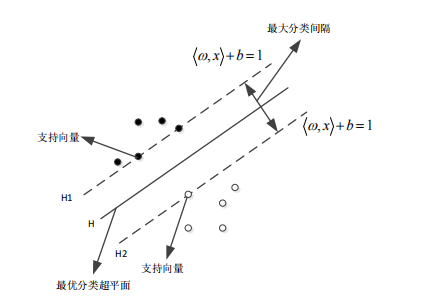
\includegraphics[width=0.5\textwidth]{svm.png}
	\caption{SVM模型原理图}
	\label{fig:svm}
\end{figure}

2、表模板
\begin{table}[htpb]
\caption{最优算法的多指标分析}
\begin{center}\label{table:score}
\begin{tabular}{|c|r|r|r|}
\hline
   & \multicolumn{1}{c|}{精确率} & \multicolumn{1}{c|}{召回率} & \multicolumn{1}{c|}{F1得分} \\ \hline
石块 & 0.94                     & 0.96                     & 0.95                      \\ \hline
金属 & 0.92                     & 0.97                     & 0.95                      \\ \hline
塑料 & 0.96                     & 0.89                     & 0.93                      \\ \hline
\end{tabular}
\end{center}
\end{table}

3、公式模板
\begin{equation}\label{eq:svmsuper}
\begin{array}{l}
\min _{\boldsymbol{w}, b} \frac{1}{2}\|\boldsymbol{w}\|^{2} \\
\text { s.t. } y_{i}\left(\boldsymbol{w}^{\mathrm{T}} \boldsymbol{x}_{i}+b\right) \geqslant 1, \quad i=1,2, \ldots, m
\end{array}
\end{equation}


4、伪代码模板
 \begin{algorithm}[H]
  \caption{ K近邻算法步骤}
  \begin{algorithmic}[1]
    \Require
      训练数据集;
      待预测数据;
    \Ensure
      预测数据的类别;
    \State 加载数据;
    \State 初始化K值;
    \State 计算预测样本与训练集中的每一个样本的距离;
    \State 将距离和索引添加到有序集合中;
    \State 对距离按从小到大排序方式对距离和索引的有序集合进行排序;
    \State 从排序的集合中选择前K条数据;
    \State 获得选的K条数据的标签;
    \State 计算每一种标签的样本数量;
    \Return 
        数量最多的标签作为样本的预测值;
  \end{algorithmic}
\end{algorithm}


5、代码模板
\lstset{language=Python}
\begin{lstlisting}
#调整图片尺寸到统一大小,并扁平化为一维数据
def image_to_feature_vector(image, size=(128, 128)):

	return cv2.resize(image, size).flatten()

#提取图像在HSV颜色空间上的颜色直方图,将直方图扁平化,
#作为特征向量返回
def extract_color_histogram(image, bins=(32, 32, 32)):
	hsv = cv2.cvtColor(image, cv2.COLOR_BGR2HSV)
	hist = cv2.calcHist([hsv], [0, 1, 2], None, bins,
		[0, 180, 0, 256, 0, 256])
	if imutils.is_cv2():
		hist = cv2.normalize(hist)
	else:
		cv2.normalize(hist, hist)
	return hist.flatten()

\end{lstlisting}
\end{appendices}

\end{document}
